\section{Neuromodulation}
In living organisms, neuromodulators are neuropeptides or small molecules, such as dopamine and
serotonin. The production of these substances within the cell is controlled by
gene regulatory networks. Neuromodulators change the behavior of neural networks
within individual neurons, amongst neighboring neurons, or throughout the entire
network. Neuromodulation has been found to be pervasive throughout the brain,
and can have drastic consequences on the behavior of neurons and neuronal
circuits \cite{Destexhe2004,Marder2012,Marder2002}. We have already noted that the temporal difference learning algorithm for error
prediction has been observed in neural substrates \cite{Schultz1993}. An
extensive review of computational models of neuromodulation can be found in
\cite{Fellous1998}, and some recent models are reviewed in \cite{Marder2012}.
In this study we extend work on the evolution of neuromodulation \cite{Soltoggio2008,Harrington2013},
focusing on the relationship between evolved neuromodulatory
GRNs and reinforcement learning \cite{Harrington2013}. 

\subsection{Regulating parameters}
With the intention of focusing on the optimization of genetically-regulated neuromodulation, the physical mechanisms underlying neuromodulation are used as inspiration and the neuromodulation of reinforcement learning was optimized. Neuromodulation has been considered in the context of RL \cite{Doya2002,Schweighofer2003,Doya2008}, but this previous work has not focused on the implications of neuromodulation on problem solving capacity. In this work we utilize the artificial gene regulatory network presented in the previous section to regulate the learning parameters of the SARSA algorithm. Three learning parameters are considered: the learning rate $\alpha$, the discount factor $\gamma$ and the memory depth $\lambda$.

To do so, the GRN uses three inputs that describe the current performance of the agent in the environment. They have been chosen to be problem-independent as one of our goals is to define a problem-independent neuromodulation architecture to minimize problem-specific adjustments. The first input describes the duration from the beginning of current episode: the concentration of this first input protein increases with the time spent in each learning episode. The concentration $C_{I_1}(t)$ of this input protein at time step $t$ is calculated as follows:
\begin{equation}
C_{I_1}(t)=e^{-\frac{t^2}{t_{max}^2}}
\end{equation}
where $t_{max}$ is the expected duration of an episode. The second output protein's concentration $C_{I_2}(t)$ describes the quality of the current sequence of actions in term of rewards, smoothed on 25 steps:
\begin{eqnarray}
C_{I_2}(t)=\frac{\sum\limits_{s=1}^{25}{\Big((25-s)\times q_s(t-1)\Big)}}{\sum\limits_{s=1}^{25}s} \\
\text{with }q_s(t)=
\begin{cases}
1+1000\frac{Q.e}{Q.Q*e.e} & \text{ if} \frac{Q.e}{Q.Q*e.e}>0.4995\\
0 & \text{ otherwise}
\end{cases}\nonumber
\end{eqnarray}
where $e$ is the eligibility trace and $Q$ is the Q-function, both described in Section \ref{sec:RL}. The aim of this input is to capture the quality of the current state history relative to previous experiences. Finally, the third input protein's concentration $C_{I_3}(t)$ informs the GRN about the 25-step smoothed average reward the agent can obtain in its current state:
\begin{equation}
C_{I_3}(t)=\frac{\sum\limits_{s=1}^{24}{\Big((25-s)\times C_{I_3}(t-s)\Big)}+25\times \sum\limits_{r_e\in e}{r_e}}{\sum\limits_{s=1}{25}s}
\end{equation}
where $e$ is the eligibility trace. This input encodes the frequency that the agent has reentered the same state. 

In addition to these inputs, the GRN uses four output proteins to regulate the learning parameters:
\begin{itemize}
\item the output protein $O_{n}$, which concentration $C_{n}$ normalizes the concentration of other outputs\footnote{This is generally used in regulatory networks to obtain output values in $[0, 1]$.},
\item the output protein $O_{\alpha}$ of concentration $C_{\alpha}$, which provides the value for $\alpha$ to the SARSA algorithm with $\alpha=C_{\alpha}/(C_\alpha+C_{n})$,
\item the output protein $O_\gamma$ of concentration $C_{\gamma}$, which provides the value for $\gamma$ to the SARSA algorithm with $\gamma=C_{\gamma}/(C_\gamma+C_{n})$,
\item the output protein $O_\lambda$ of concentration $c_{\lambda}$, which provides the value for $\lambda$ to the SARSA algorithm with $\lambda=C_{\lambda}/(C_\lambda+C_{n})$.
\end{itemize}

As depicted by figure \ref{fig:GRNSARSA}, the GRN updates SARSA's learning parameters at every time step, before SARSA updates its internal variables and prediction. The GRN returns the learning parameters SARSA uses for its own decision step.

\begin{figure}
\center
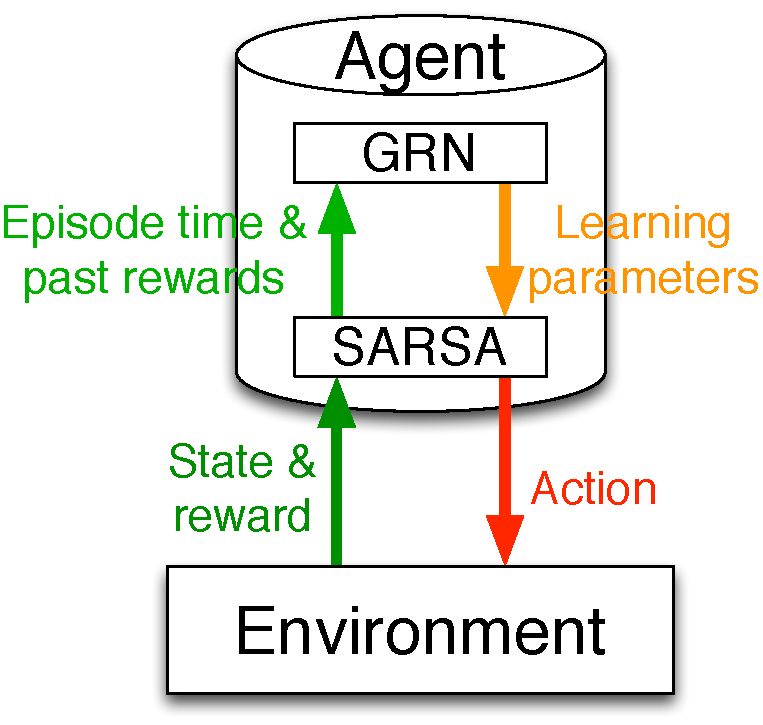
\includegraphics[width=0.7\linewidth]{GRNSARSA.pdf}
\caption{At every time step, SARSA updates the GRN inputs. The GRN returns updated learning parameters that will be used by the SARSA algorithm.}\label{fig:GRNSARSA}
\end{figure}

%%% Problem figure from experiences %%%
\begin{figure*}[ht!]
\begin{minipage}[t]{0.31\linewidth}
\center
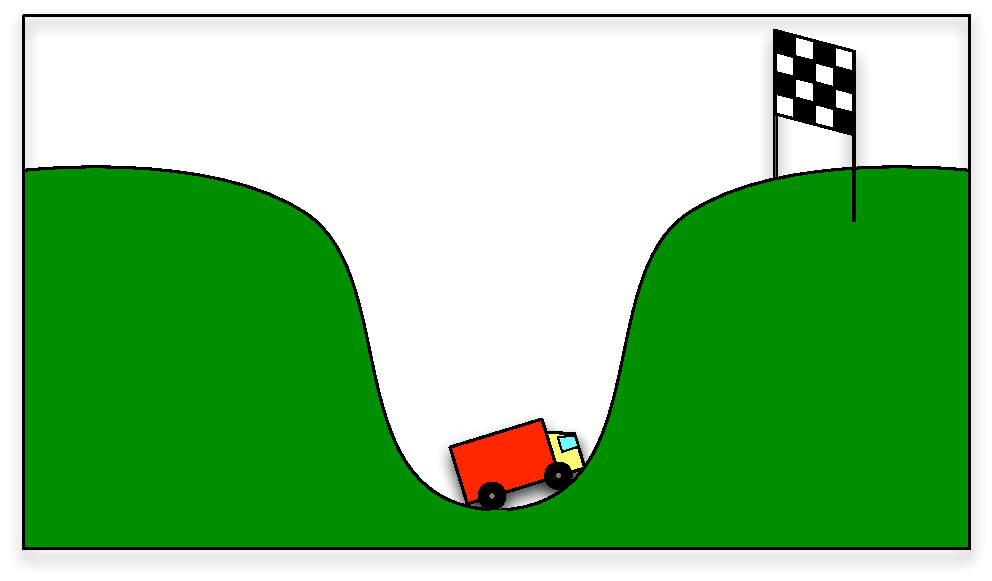
\includegraphics[height=3.2cm]{MC_problem.pdf}
\caption{Mountain car
%In the mountain car problem, a car must escape from a valley. It cannot climb the hill without moving backward first to gain speed. The agent receives a reward only when it escapes.
}\label{fig:MC:problem}
\end{minipage}
\hspace{0.1mm}
\begin{minipage}[t]{0.25\linewidth}
\center
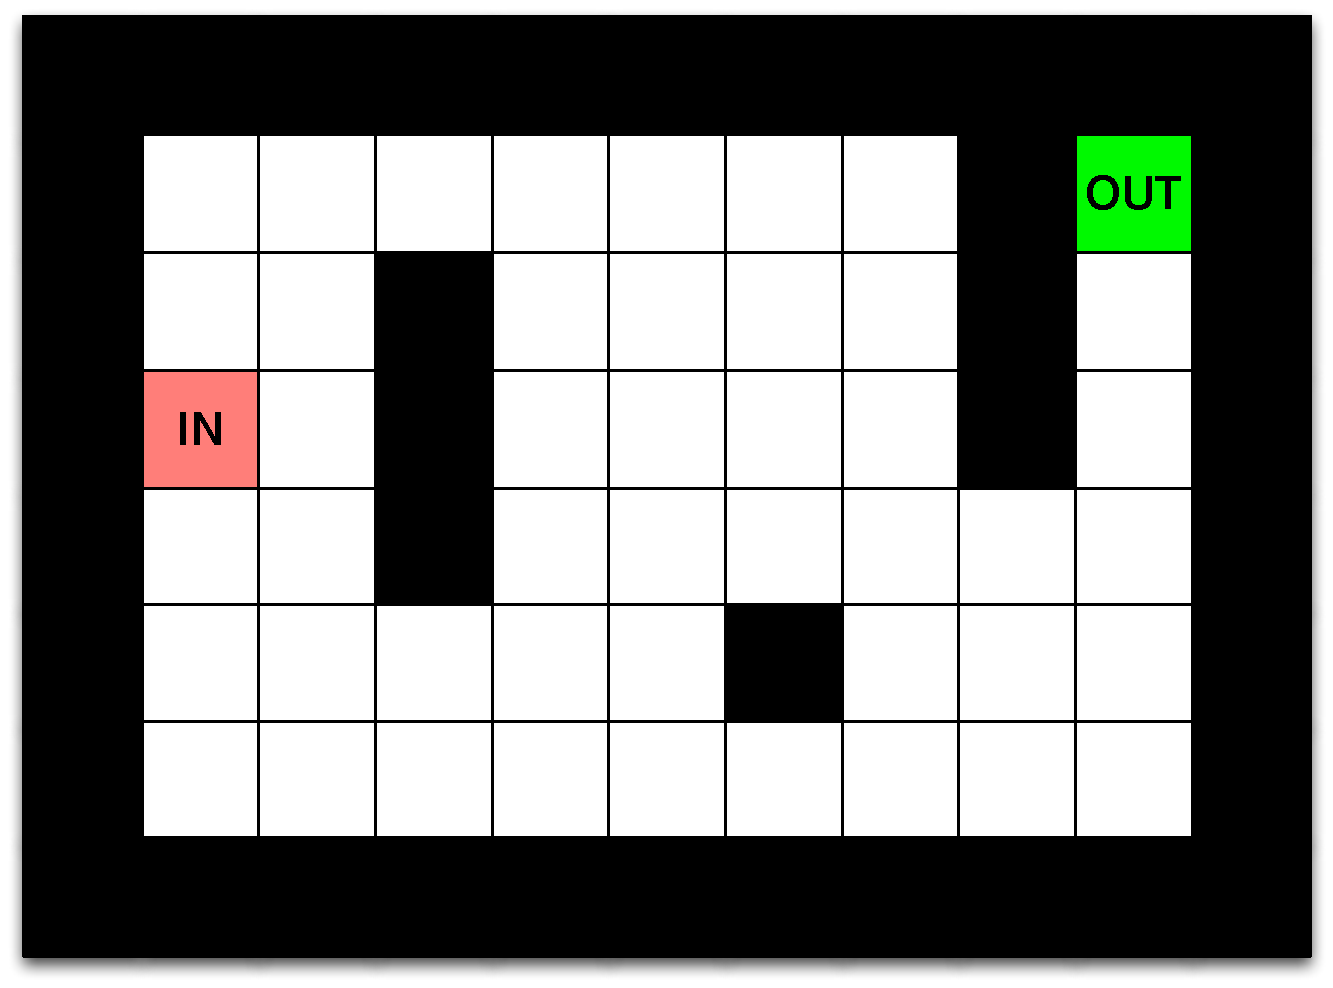
\includegraphics[height=3.2cm]{MZ_problem.pdf}
\caption{Maze
%In the maze problem, the agent's task is to find its way in a maze from start (in red) to finish (in green). The agent receives a reward only when it escapes.
}\label{fig:MZ:problem}
\end{minipage}
\hspace{0.1mm}
\begin{minipage}[t]{0.22\linewidth}
\center
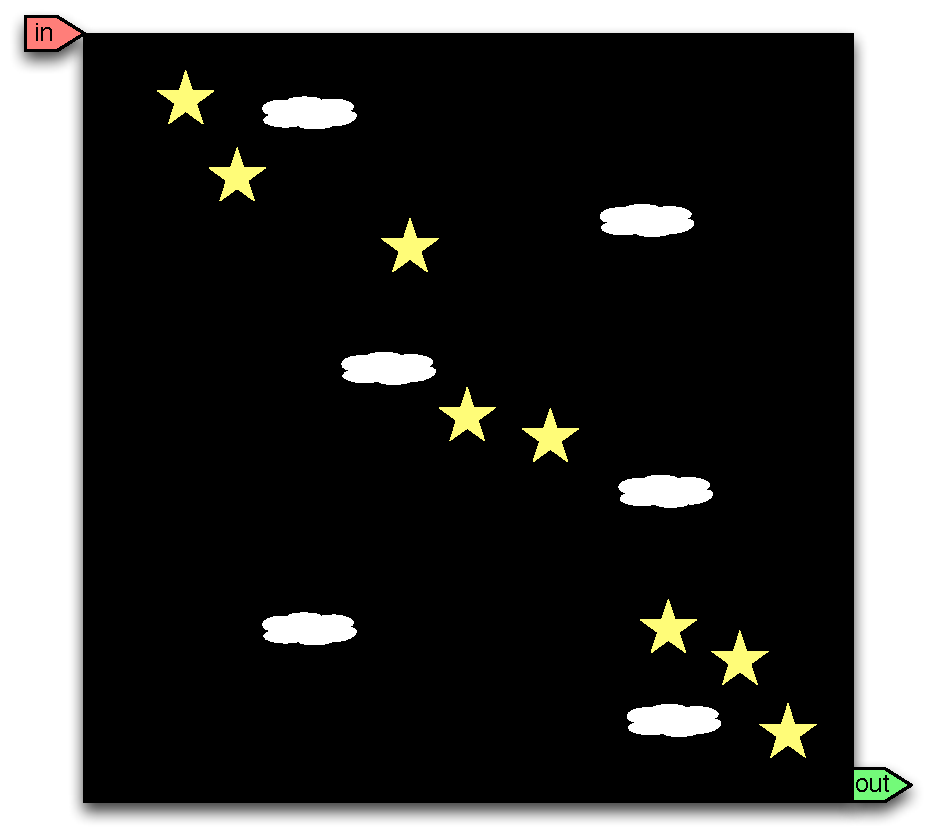
\includegraphics[height=3.2cm]{PW_problem.pdf}
\caption{Puddle world
%In the puddle world problem, the agent must navigate without sensor information with stochastic movements from start to finish. Rewards are given all along its exploration (stars) and when it escapes.
}\label{fig:PW:problem}
\end{minipage}
\hspace{0.1mm}
\begin{minipage}[t]{0.19\linewidth}
\center
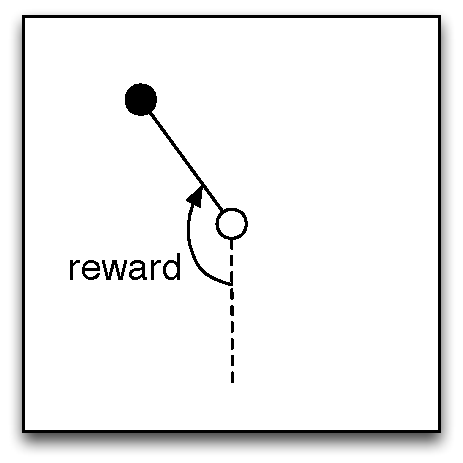
\includegraphics[height=3.2cm]{ACP_problem.pdf}
\caption{Acrobat
%In the acrobat problem, the agent has to balance a pendulum in a perfectly upright position. The reward is given by the cosine of the angle between the pendulum and the resting position.
}\label{fig:ACP:problem}
\end{minipage}
\end{figure*}

\subsection{GRN Optimization}
Before a gene regulatory network can be used for successful neuromodulation, the GRN must be optimized. In this paper, we use an evolutionary algorithm inspired by the NEAT algorithm \cite{stanley2002evolving}, but adapted for GRNs called GRNEAT \cite{cussatblanc2015grneat}. GRNEAT incorporates three key features:
\begin{itemize}
\item \emph{initialization} of the algorithm  - as opposed to initializing with network sizes randomly sampled from the complete distribution, only small networks are used in the initial population so as to allow for a more progressive complexification,
\item \emph{speciation} protects newly appeared solutions by giving them some time to optimize their structures before competing with the whole population, and
\item \emph{alignment crossover} uses of a distance metric between proteins to maintain subnetwork architecture during the crossover operation.
\end{itemize}
This modified algorithm has been shown to converge faster and to better solutions than standard genetic algorithms. More details on GRNEAT can be found in \cite{cussatblanc2015grneat}.

During optimization, each GRN is evaluated independently on a given problem with 25 reruns in order to reduce the effect of stochasticity on fitness. As fitness is problem dependent, more detail is provided in the corresponding experiment sections. To avoid any memory bias, SARSA is completely reset before each evaluation. The parameters used for GRNEAT in this work are given by Table~\ref{tab:GREAT:params}, and are consistent for all problems. 

\begin{table}
\center
\begin{tabular}{rl}
Parameter			& value 					\\\hline
Population size		& 500					\\
Initial duplicates		& 19					\\
Speciation threshold 	& 0.15					\\
Species min size		& 15					\\
Selection				& 3-players tournament	\\
Crossover rate		& 0.2					\\
Mutation rate			& 0.8					\\
\end{tabular}
\caption{GRNEAT parameters used for evolution.}\label{tab:GREAT:params}
\end{table}



